% Created 2024-03-20 Wed 10:26
% Intended LaTeX compiler: lualatex
\documentclass[xcolor=table,10pt,aspectratio=169]{beamer}

\RequirePackage[l2tabu,orthodox]{nag}            %% Warn about obsolete commands and packages
\RequirePackage{amsmath,amsfonts,amssymb,amsthm} %% Math
\RequirePackage{ifpdf,ifxetex,ifluatex}          %% Detect XeTeX and LuaTeX
\RequirePackage{xspace}
\RequirePackage{graphicx}
\RequirePackage{comment}
\RequirePackage{url}
\RequirePackage{relsize}
\RequirePackage{booktabs}
\RequirePackage{tabularx}
\RequirePackage[normalem]{ulem}
\ifluatex%
\else%
  \RequirePackage[all]{xy}
\fi%
\RequirePackage{etoolbox}
\RequirePackage{csquotes}
\RequirePackage[export]{adjustbox}

\RequirePackage{silence}
\WarningsOff[microtype]
\WarningFilter{microtype}{Unknown slot}

% https://tex.stackexchange.com/questions/64459/overfull-vbox-warning-disable
\vfuzz=30pt
\hfuzz=30pt


%%%
%%% Code Listings
%%%

\RequirePackage{listings}
\lstdefinelanguage{Sage}[]{Python}{morekeywords={True,False,sage,cdef,cpdef,ctypedef,self},sensitive=true}

\lstset{frame=none,
  showtabs=False,
  showspaces=False,
  showstringspaces=False,
  commentstyle={\color{gray}},
  keywordstyle={\color{mLightBrown}\textbf},
  stringstyle ={\color{mDarkBrown}},
  frame=single,
  basicstyle=\tt\scriptsize\relax,
  backgroundcolor=\color{gray!190!black},
  inputencoding=utf8,
  literate={…}{{\ldots}}1,
  belowskip=0.0em,
}

\makeatletter
\patchcmd{\@verbatim}
  {\verbatim@font}
  {\verbatim@font\scriptsize}
  {}{}
\makeatother


%%%
%%% Pseudocode
%%%

\let\nl\undefine
\let\procedure\relax
\let\endprocedure\relax
\usepackage{algorithm2e}

%%%
%%% Tikz
%%%

\RequirePackage{tikz,pgfplots}
\pgfplotsset{compat=newest}

\usetikzlibrary{calc}
\usetikzlibrary{arrows}
\usetikzlibrary{automata}
\usetikzlibrary{positioning}
\usetikzlibrary{decorations.pathmorphing}
\usetikzlibrary{backgrounds}
\usetikzlibrary{fit,}
\usetikzlibrary{shapes.symbols}
\usetikzlibrary{chains}
\usetikzlibrary{shapes.geometric}
\usetikzlibrary{shapes.arrows}
\usetikzlibrary{graphs}

%% Cache but disable by default

\usetikzlibrary{external}
\tikzset{external/export=false}

\definecolor{DarkPurple}{HTML}{332288}
\definecolor{DarkBlue}{HTML}{6699CC}
\definecolor{LightBlue}{HTML}{88CCEE}
\definecolor{DarkGreen}{HTML}{117733}
\definecolor{DarkRed}{HTML}{661100}
\definecolor{LightRed}{HTML}{CC6677}
\definecolor{LightPink}{HTML}{AA4466}
\definecolor{DarkPink}{HTML}{882255}
\definecolor{LightPurple}{HTML}{AA4499}
\definecolor{DarkBrown}{HTML}{604c38}
\definecolor{DarkTeal}{HTML}{23373b}
\definecolor{LightBrown}{HTML}{EB811B}
\definecolor{LightGreen}{HTML}{14B03D}
\definecolor{DarkOrange}{HTML}{FFDD00}

\pgfplotsset{width=1.0\textwidth,
  height=0.6\textwidth,
  cycle list={%
    solid,LightGreen,thick\\%
    dotted,LightRed,very thick\\%
    dashed,DarkBlue,thick\\%
    dashdotted,DarkPink,thick\\%
    dashdotdotted,LightGreen,thick\\%
    loosely dotted,very thick\\%
    loosely dashed,DarkBlue,very thick\\%
    loosely dashdotted,DarkPink,very thick\\%
    \\%
    DarkBrown,thick\\%
  },
  legend pos=north west,
  legend cell align={left}}

\pgfplotsset{select coords between index/.style 2 args={
    x filter/.code={
        \ifnum\coordindex<#1\def\pgfmathresult{}\fi
        \ifnum\coordindex>#2\def\pgfmathresult{}\fi
    }
}}

\setlength{\marginparwidth}{2cm}
\pgfplotsset{compat=1.18}

%%%
%%% SVG (Inkscape)
%%%

\ifpdf% 
\providecommand{\executeiffilenewer}[3]{%
  \ifnum\pdfstrcmp{\pdffilemoddate{#1}}%
    {\pdffilemoddate{#2}}>0%
    {\immediate\write18{#3}}
  \fi%
}
\else%
\providecommand{\executeiffilenewer}[3]{%
  {\immediate\write18{#3}} % hack
}
\fi%

\providecommand{\includesvg}[2][1.0\textwidth]{%
 \executeiffilenewer{#1.svg}{#1.pdf}%
 {inkscape -z -D --file=#2.svg --export-pdf=#2.pdf --export-latex --export-area-page}%
 \def\svgwidth{#1} 
 \input{#2.pdf_tex}%
} 

%%%
%%% Attachments
%%%

\RequirePackage{embedfile}


%%%
%%% Metropolis Theme
%%%

\usetheme{metropolis}
\metroset{color/block=fill}
\metroset{numbering=none}
\metroset{outer/progressbar=foot}
\metroset{titleformat=smallcaps}

\setbeamercolor{description item}{fg=mLightBrown}
\setbeamerfont{footnote}{size=\scriptsize}
\setbeamercolor{example text}{fg=mDarkBrown}
\setbeamercolor{block title alerted}{fg=white, bg=mDarkBrown}
\setbeamerfont{alerted text}{series=\ifmmode\boldmath\else\bfseries\fi}

\renewcommand*{\UrlFont}{\ttfamily\relax}

%%%
%%% UTF-8 & Fonts
%%% 

\RequirePackage{unicodesymbols} % after metropolis which loads fontspec

\ifboolexpr{bool{xetex} or bool{luatex}}{%
\setmonofont[BoldFont={Cousine Bold},
             ItalicFont={Cousine Italic},
             BoldItalicFont={Cousine Bold Italic},
             Scale=0.9]{Cousine}             
}{%
}

%%%
%%% BibLaTeX
%%%

\RequirePackage[backend=bibtex,
            style=alphabetic,
            maxnames=8,maxbibnames=8,maxalphanames=8,
            citestyle=alphabetic]{biblatex}

\bibliography{local.bib,abbrev3.bib,crypto_crossref.bib,rfc.bib,jacm.bib,dcc.bib}

\setbeamertemplate{bibliography item}[text]
% https://tex.stackexchange.com/questions/683533/beamer-theme-metropolis-does-not-allow-different-font-size-for-fullcite
\setbeamerfont{bibliography entry title}{size=}
\setbeamerfont{bibliography entry author}{size=}
\setbeamerfont{bibliography entry location}{size=}
\setbeamerfont{bibliography entry note}{size=}

\DeclareFieldFormat{title}{\alert{#1}}
\DeclareFieldFormat[book]{title}{\alert{#1}}
\DeclareFieldFormat[thesis]{title}{\alert{#1}}
\DeclareFieldFormat[inproceedings]{title}{\alert{#1}}
\DeclareFieldFormat[incollection]{title}{\alert{#1}}
\DeclareFieldFormat[article]{title}{\alert{#1}}
\DeclareFieldFormat[misc]{title}{\alert{#1}}

%%% 
%%% Microtype
%%%

\IfFileExists{upquote.sty}{\RequirePackage{upquote}}{}
\IfFileExists{microtype.sty}{\RequirePackage{microtype}}{}
\IfFileExists{microtype.sty}{\PassOptionsToPackage{verbose=silent}{microtype}}{}

\setlength{\parindent}{0pt}                   %%
\setlength{\parskip}{6pt plus 2pt minus 1pt}  %%
\setlength{\emergencystretch}{3em}            %% prevent overfull lines
\setcounter{secnumdepth}{0}                   %%

%%%
%%% Maths
%%%

\DeclareMathOperator{\Vol}{Vol}
\DeclareMathOperator{\GH}{GH}
\renewcommand{\vec}[1]{\ensuremath{\mathbf{#1}}\xspace}
\newcommand{\norm}[1]{\left\lVert#1\right\rVert}
\providecommand{\mat}[1]{\ensuremath{\vec{#1}}\xspace}
\providecommand{\ring}[0]{\ensuremath{\mathcal{R}}\xspace}


\usepackage{graphicx}
\usepackage{longtable}
\usepackage{wrapfig}
\usepackage{rotating}
\usepackage[normalem]{ulem}
\usepackage{amsmath}
\usepackage{amssymb}
\usepackage{capt-of}
\usepackage{hyperref}
\usepackage{booktabs}
\usepackage{microtype}
\usepackage{newunicodechar}
\usepackage[notions,operators,sets,keys,ff,adversary,primitives,complexity,asymptotics,lambda,landau,advantage]{cryptocode}
\usepackage[capitalize]{cleveref}
\usepackage[,]{stmaryrd}
\usepackage[american]{babel}
\usepackage{xspace}
\usepackage{units}
\usepackage{nicefrac}
\usepackage{gensymb}
\usepackage{amsthm}
\usepackage{amsmath}
\usepackage{amssymb}
\usepackage{xcolor}
\usepackage{listings}
\usepackage[color=cyan!0!magenta!4!yellow!16]{todonotes}
\PassOptionsToPackage{british}{babel}
\setbeamerfont{alerted text}{series=\ifmmode\boldmath\else\bfseries\fi}
% \tikzset{external/export=true}
\institute{King's College London \& SandboxAQ}
\usepackage{newunicodechar}
\newfontfamily{\fallbackfont}{DejaVu Sans}
\DeclareTextFontCommand{\textfallback}{\fallbackfont}
\newcommand{\fallbackchar}[2][\textfallback]{\newunicodechar{#2}{#1{#2}}}
\fallbackchar{↻}
\usepackage{luacolor}
\usepackage{lua-ul}
\definecolor{BrightOrange}{HTML}{f8e8c6}
\usetheme{default}
\author{Martin R. Albrecht}
\date{RWPQC}
\title{An Update on Lattice Cryptanalysis Vol. 1}
\subtitle{The Dual Attack on LWE}
\hypersetup{
pdfauthor={Martin R. Albrecht},
pdftitle={An Update on Lattice Cryptanalysis Vol. 1},
pdfkeywords={},
pdfsubject={},
pdfcreator={Emacs 29.2.50 (Org mode 9.6.15)},
pdflang={English},
colorlinks,
citecolor=gray,
filecolor=gray,
linkcolor=gray,
urlcolor=gray
}
\begin{document}

\maketitle



\begin{frame}[label={sec:orgef6af93}]{Kyber}
\begin{columns}[t]
\begin{column}{0.5\columnwidth}
\begin{center}
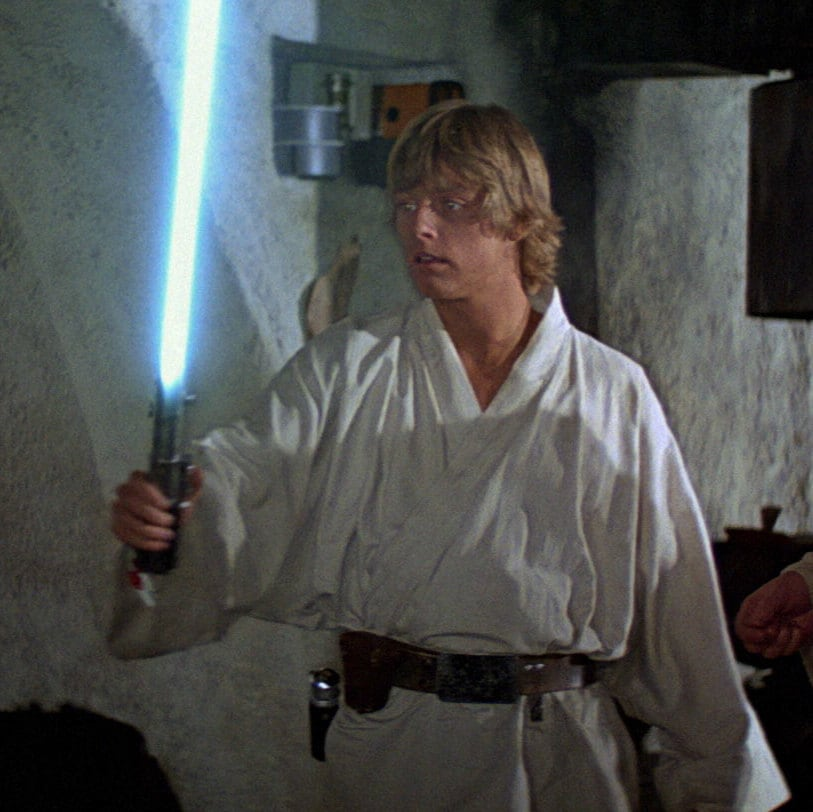
\includegraphics[keepaspectratio,height=.75\textheight]{./lightsaber.jpeg}
\end{center}
\end{column}

\begin{column}{0.5\columnwidth}
\begin{center}
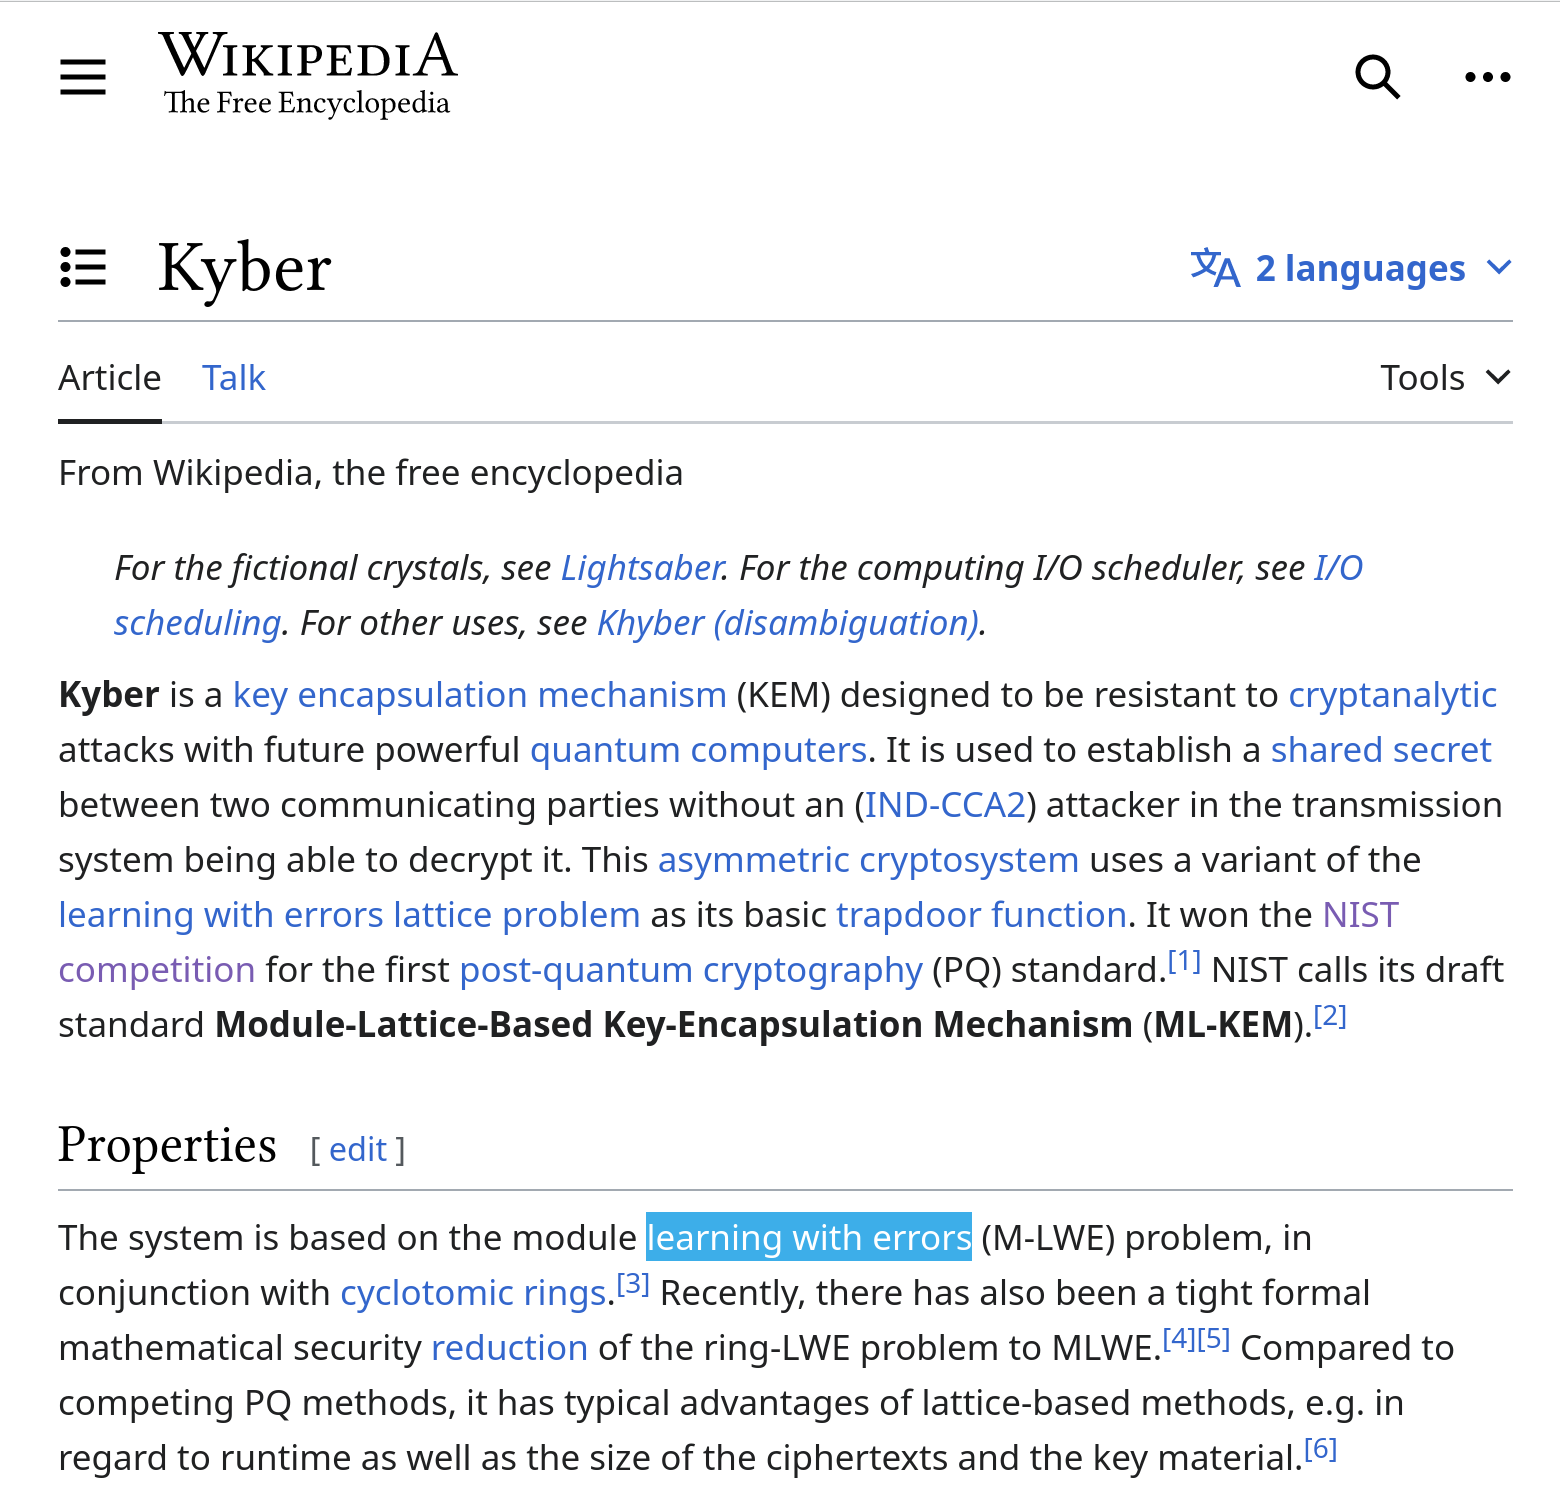
\includegraphics[keepaspectratio,height=.75\textheight]{./kyber.png}
\end{center}
\end{column}
\end{columns}

The reason you cannot find information about lightsaber crystals any longer …
\end{frame}

\begin{frame}[label={sec:org9e56893}]{Learning with Errors}
\begin{columns}
\begin{column}[t]{0.6\columnwidth}
Given \((\mat{A},\vec{c}) \in \ZZ_{q}^{m \times n} \times \ZZ_{q}^{m}\), find \(\vec{s}  \in \ZZ^{n}\) when

\[
\left(\begin{array}{c} \\ \\ \\ \vec{c}\\ \\ \\ \\ \end{array} \right)
\equiv \left(\begin{array}{ccc}
\leftarrow & n & \rightarrow \\ \\ \\ 
& \mathbf{A} & \\
\\ \\ \\
\end{array} \right)
\cdot \left(\begin{array}{c} \\ \\ \vec{s}\\ \\ \\ \end{array} \right)
+ \left(\begin{array}{c} \\ \\ \\ \vec{e}\\ \\ \\ \\\end{array}\right)
\bmod q
\]

for \(\vec{e} \in \ZZ^{m}\) with small entries.

\begin{alertblock}{Example}
\(n = 1024, m=2048, q=7681, |e_{i}| \approx 2\)
\end{alertblock}
\end{column}

\begin{column}[t]{0.4\columnwidth}
\begin{block}{``Small Entries''}
\begin{tikzpicture}
  \begin{axis}[
    domain=-10:10,
    grid=major,smooth,
    % xlabel=$x$,
    % ylabel=$\approx \textnormal{Pr}(x)$,
    ]
    \addplot[color=LightBrown,thick,samples=50,smooth]{exp(-(x^2)/18)};
    \addplot[color=DarkBrown,only marks] coordinates {
      (-9, 0.011)
      (-8, 0.028)
      (-7, 0.065)
      (-6, 0.135)
      (-5, 0.249)
      (-4, 0.411)
      (-3, 0.606)
      (-2, 0.800)
      (-1, 0.945)
      (0, 1.000)
      (1, 0.945)
      (2, 0.800)
      (3, 0.606)
      (4, 0.411)
      (5, 0.249)
      (6, 0.135)
      (7, 0.065)
      (8, 0.028)
      (9, 0.011)
    };
  \end{axis}
\end{tikzpicture}
\end{block}

No loss in security if secret \(\vec{s}\) and error \(\vec{e}\) have same distribution \cite{C:ACPS09}
\end{column}
\end{columns}
\end{frame}

\begin{frame}[label={sec:orgddf3dd0}]{Primal Attack}
\begin{columns}
\begin{column}[t]{0.7\columnwidth}
We can reformulate \(\vec{c} - \mat{A} \cdot \vec{s} \equiv \vec{e} \bmod q\)  over the Integers as:
\[
    \begin{pmatrix}q\mat{I} & -\mat{A}\\0 & \mat{I}\\\end{pmatrix}
  \cdot \begin{pmatrix}\vec{*}\\\vec{s}\end{pmatrix}
  + \begin{pmatrix}\vec{c}\\\vec{0}\end{pmatrix}
  = \begin{pmatrix}\vec{e}\\\vec{s}\end{pmatrix}
\]
Alternatively:
\[
  \mat{B} = \begin{pmatrix}q\mat{I} & -\mat{A} & \vec{c}\\
  0 & \mat{I} & 0\\
  0 & 0 & 1\\
  \end{pmatrix}
  , \qquad
  \mat{B}
  \cdot \begin{pmatrix}\vec{*}\\\vec{s}\\1\end{pmatrix}
  = \begin{pmatrix}\vec{e}\\\vec{s}\\1\end{pmatrix}
\]

\begin{block}{A Unique Shortest Vector}
There exists an integer-linear combination of the columns of \(\mat{B}\) that produces a vector with “unusually” small entries
\end{block}
\end{column}

\begin{column}[t]{0.3\columnwidth}
\begin{alertblock}{uSVP}
Find a unique shortest vector amongst the integer combinations of the columns of:
\[
  \mat{B} = \begin{pmatrix}
 q\mat{I} & -\mat{A} & \vec{c}\\
 0        & \mat{I}  & 0\\
 0        & 0        & 1\\
  \end{pmatrix}
\]
where \(\mat{B} \in \ZZ^{d \times d}\).
\end{alertblock}
\end{column}
\end{columns}
\end{frame}

\begin{frame}[label={sec:org5b344e8}]{Dual Attack}
\begin{columns}
\begin{column}{0.6\columnwidth}
\begin{itemize}
\item Consider \(\vec{c} \equiv \mat{A} \cdot \vec{s} + \vec{e} \bmod q\) with both \(\vec{s}\) and \(\vec{e}\) short or \(\vec{c}\) uniform.
\item Let \(\vec{u}\) be short such that \(\vec{v}^{T} \coloneqq \vec{u}^{T} \cdot \mat{A} \bmod q\)  is short.
\item Compare:
\begin{itemize}
\item \(\vec{u}^{T} \cdot \vec{c} \equiv \vec{u}^{T} \cdot \vec{A} \cdot \vec{s} + \vec{u}^{T} \cdot \vec{e} \equiv \vec{v}^{T} \cdot \vec{s} + \vec{u}^{T}\cdot \vec{e}\)  \(\Rightarrow\) \alert{short-ish}
\item \(\vec{u}^{T} \cdot \vec{c}\) \(\Rightarrow\) \alert{uniform}
\end{itemize}
\item The shorter \((\vec{u},\vec{v})\) the fewer \(\vec{u}^{T} \cdot \vec{c}\) we need
\item Note
\end{itemize}
\[
  \begin{pmatrix}
    q\mathbf{I} & \mathbf{A}^{T}\\
    0 & \mathbf{I}\\
  \end{pmatrix} \cdot
  \begin{pmatrix}
    \vec{*}\\
    \vec{u}
  \end{pmatrix} = 
  \begin{pmatrix}
    \vec{v}\\
    \vec{u}
  \end{pmatrix}  
\]
\end{column}

\begin{column}{0.4\columnwidth}
\begin{alertblock}{Approx-SVP}
Find vectors \((\vec{u}_i, \vec{v}_i)\) of norm \(\|(\vec{u}_i, \vec{v}_i)\| \leq \beta\) amongst the integer combinations of the columns of \(\mat{B} \in \ZZ^{d \times d}\):
\[
  \mat{B} = \begin{pmatrix}
 q\mat{I} & \mat{A}^{T}\\
 0        & \mat{I}\\
  \end{pmatrix}
\]
\end{alertblock}

Can extend this to recover \(\vec{s}\): guess a component and run the distinguisher
\end{column}
\end{columns}
\end{frame}

\begin{frame}[label={sec:org1949319},fragile]{Why we're here I}
 \textbf{NIST's ask:}

\begin{center}
\begin{tabular}{ll}
\toprule
AES 128 & \(2^{170}\)/MAXDEPTH quantum gates or \(\mathbf{2^{143}}\) classical gates\footnotemark\\[0pt]
\bottomrule
\end{tabular}

\end{center}\footnotetext[1]{\label{org0b558d0}``\emph{In particular, NIST will define a separate category for each of the following security requirements (listed in order of increasing strength): 1) Any attack that breaks the relevant security definition must require computational resources comparable to or greater than those required for key search on a block cipher with a 128-bit key (e.g. AES128)}'' \fullcite{NISTPQC17}}

\textbf{Current estimates:}

\begin{lstlisting}[language=Python,label= ,caption= ,captionpos=b,numbers=none]
from estimator import *
_ = LWE.estimate(schemes.Kyber512)
\end{lstlisting}

\begin{verbatim}
bkw                  :: rop: ≈2^178.8, m: ≈2^166.8, mem: ≈2^167.8, b: 14, t1: 0, t2: 16, ...
usvp                 :: rop: ≈2^143.8, red: ≈2^143.8, δ: 1.003941, β: 406, d: 998, tag: usvp
bdd                  :: rop: ≈2^140.3, red: ≈2^139.7, svp: ≈2^138.8, β: 391, η: 421, d: 1013, tag: bdd
dual                 :: rop: ≈2^149.9, mem: ≈2^97.1, m: 512, β: 424, d: 1024, ↻: 1, tag: dual
dual_hybrid          :: rop: ≈2^139.2, red: ≈2^139.0, guess: ≈2^136.2, β: 385, p: 6, ζ: 15, ...
\end{verbatim}

\begin{center}
\alert{{139.2 < 143}}
\end{center}
\end{frame}

\begin{frame}[label={sec:org6645cd2}]{Why we're here II}
\begin{quote}
\textbf{Ethical considerations.} Although Picante demonstrates significant progress towards attacking real-world LWE problems with sparse binary secrets, \alert{it cannot yet break} problems with real-world-size parameters. In particular, the LWE schemes standardized by NIST use smaller modulus q and non-sparse secret distributions. Hence, we do not believe our paper raises any ethical concerns. Nonetheless, we shared a copy of the current paper with the NIST Cryptography group, to inform them of our approach.
\end{quote}

\begin{itemize}
\item {\footnotesize \fullcite{CCS:LSWMGCL23} \par}
\end{itemize}
\end{frame}

\begin{frame}[label={sec:org592ac25}]{Programme}
\begin{columns}[t]
\begin{column}{0.45\columnwidth}
\textbf{This Talk:}

\begin{itemize}
\item Higher-level discussion of the ``dual attack'' which seems to come out on top in security estimates
\item Discussion of ML attacks on LWE
\end{itemize}
\end{column}

\begin{column}{0.55\columnwidth}
\textbf{John's Talk:}

\begin{itemize}
\item Opening the box of the underlying algorithm for finding short vectors (sieving) and its costs
\end{itemize}
\end{column}
\end{columns}
\end{frame}

\begin{frame}[label={sec:org564a4cc}]{Dual-Sieve Attacks}
\begin{columns}
\begin{column}[t]{0.47\columnwidth}
\textbf{An Abridged History of …}

\begin{itemize}
\item \cite{Aharonov:2005:LPN} use short vectors to distinguish
\item \cite{USENIX:ADPS16} a lattice sieve \textbf{yields many short vectors}
\item \cite{EC:Albrecht17} guess \textbf{multiple coordinates} of the secret and \textbf{reuse reduced bases}
\item \cite{AC:GuoJoh21} speed up evaluating distinguisher with a Fast Fourier Transform (FFT)
\item \cite{Matzov22} improve dual attack with modulus switching technique
\end{itemize}
\end{column}

\begin{column}[t]{0.53\columnwidth}
\textbf{… Dual-Sieve Attacks, Reconsidered}

\footnotesize

\begin{itemize}
\item \fullcite{EPRINT:DucPul23}
\item \fullcite{EPRINT:PouShe23}
\item \fullcite{EPRINT:DucPul23b}
\end{itemize}

\par
\end{column}
\end{columns}
\end{frame}

\begin{frame}[label={sec:orgeba1d45}]{Dual-Sieve Attacks}
\begin{itemize}
\item Consider \(\vec{c} \equiv \mat{A} \cdot \vec{s} + \vec{e} \bmod q\) with both \(\vec{s}\) and \(\vec{e}\) short or \(\vec{c}\) uniform.
\item Write \(\vec{s} = (\vec{s}_{\ell}, \vec{s}_{g})\) and \(\mat{A} = [\mat{A}_{\ell} \mid \mat{A}_{g}]\)
\item Let \(\vec{u}_{i}\) be short such that \(\vec{v}_i^{T} \coloneqq \vec{u}_i^{T} \cdot \mat{A}_{\ell} \bmod q\)  is short.
\item Pressing the ``sieve'' button once gives us exponentially many such vectors.
\item We have
\(
\vec{u}_i^{T} \cdot \vec{c}
\equiv \vec{u}_i^{T} \cdot (\vec{A}_{\ell} \cdot \vec{s}_{\ell} + \vec{A}_{g} \cdot \vec{s}_{g})  + \vec{u}_i^{T} \cdot \vec{e}
\equiv \vec{v}_i^{T} \cdot \vec{s}_{\ell} + \vec{u}_i^{T} \cdot \vec{A}_{g} \cdot \vec{s}_{g} +  \vec{u}_i^{T}\cdot \vec{e}
\)
\item Let \(\tilde{\vec{s}}_{g}\) be a guess for \(\vec{s}_{g}\) and consider
  \[
  \vec{v}^{T} \cdot \vec{s}_{\ell} + \vec{u}_i^{T} \cdot \vec{A}_{g} \cdot \vec{s}_{g} \highLight[BrightOrange]{- \vec{u}_i^{T} \cdot \vec{A}_{g} \cdot \tilde{\vec{s}}_{g}} + \vec{u}_i^{T}\cdot \vec{e}
  \equiv \vec{v}_i^{T} \cdot \vec{s}_{\ell}
  + \highLight[BrightOrange]{\vec{u}_i^{T} \cdot \vec{A}_{g} \cdot \left(\vec{s}_{g} - \tilde{\vec{s}}_{g}\right)}
  + \vec{u}_i^{T}\cdot \vec{e}
\]\vspace{-\baselineskip}
\item Correct guess: \textbf{small-ish} value; incorrect guess \textbf{uniform-ish} value.
\item Score guesses by sums of these values for different \((\vec{v}_i, \vec{u}_i)\)
\end{itemize}
\end{frame}

\begin{frame}[label={sec:org072f57d}]{``Small-ish'' and ``Uniform-ish'' Unpacked}
\begin{columns}
\begin{column}{0.5\columnwidth}
Success depends on the geometry of
\[
\Lambda \subset \Lambda_{q}^{\bot}(\mat{A}_{\ell})  = \{\vec{u} \in \ZZ^{m} \mid \vec{u}^{T} \cdot \mat{A}_{\ell} \equiv \vec{0} \bmod q\},
\]
lattice spanned by outputs of the sieve.

\begin{itemize}
\item We are asking our correct guess to ``win'' against all wrong guesses for \(\tilde{\vec{s}}_{g}\)
\item ``Winning'' means being closer to \(\Lambda\)
\item \cite{EPRINT:DucPul23} shows that this goes wrong when modelling the outcome of the wrong guesses as uniformly random
\item Given enough targets there will be random targets that are closer to \(\Lambda\) than the correct \(\Rightarrow\) ``contradictory regime''
\end{itemize}
\end{column}


\begin{column}{0.5\columnwidth}
\begin{center}
\textbf{Follow-up work}
\end{center}

\begin{center}
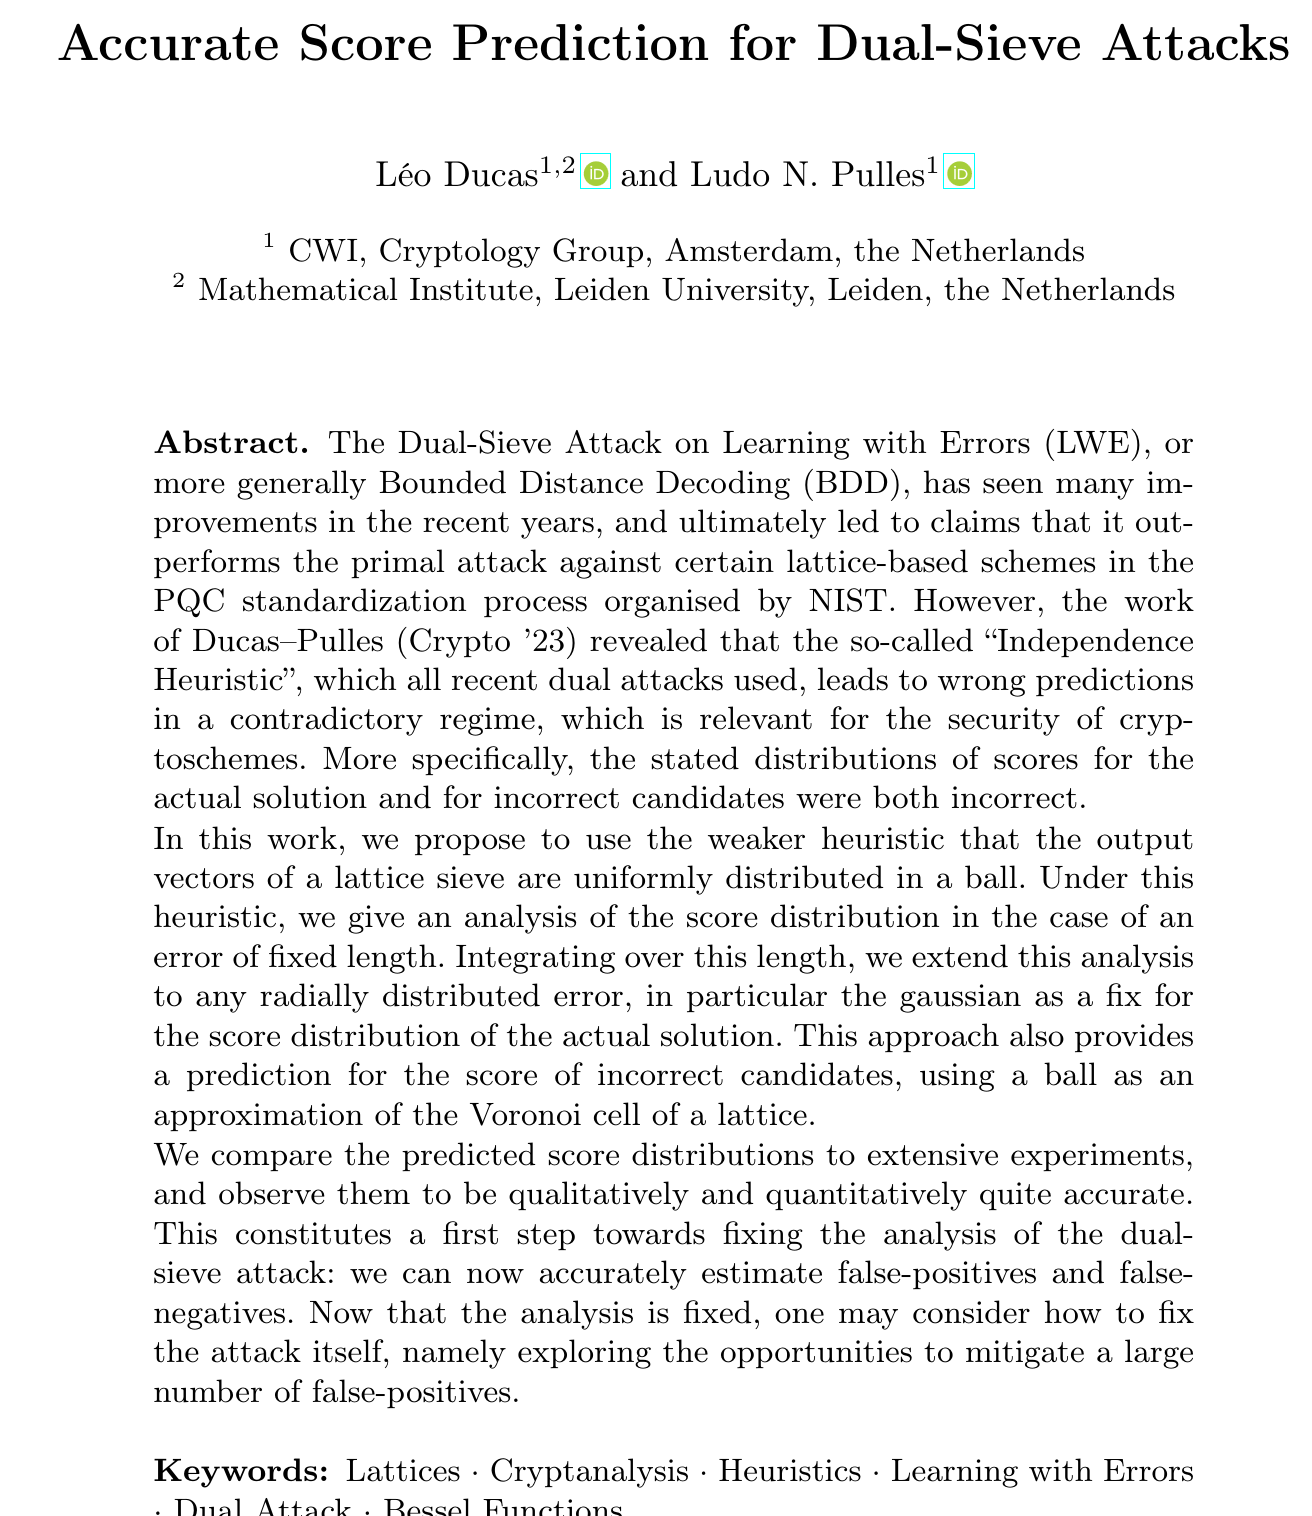
\includegraphics[keepaspectratio,height=.75\textheight]{./ludo.png}
\end{center}
\end{column}
\end{columns}
\end{frame}

\begin{frame}[label={sec:orgaf2ab97}]{Alternative Approach}
\begin{columns}
\begin{column}{0.55\columnwidth}
\begin{itemize}
\item Starts over and proves a variant of the dual attack \textbf{without any statistical assumption}
\item Does not model/prove ``modulus switching'' which greatly reduces guessing cost.
\item Provable variant works in a regime that complements the contradictory regime of \cite{EPRINT:DucPul23}
\item \textbf{Caveat:} premises of provable variant and of contradictory regime differ
\item Work also gives a guestimate of what this attack with modulus-switching added could cost (spoiler: similar to costs of \cite{Matzov22}.)
\end{itemize}
\end{column}

\begin{column}{0.45\columnwidth}
\begin{center}
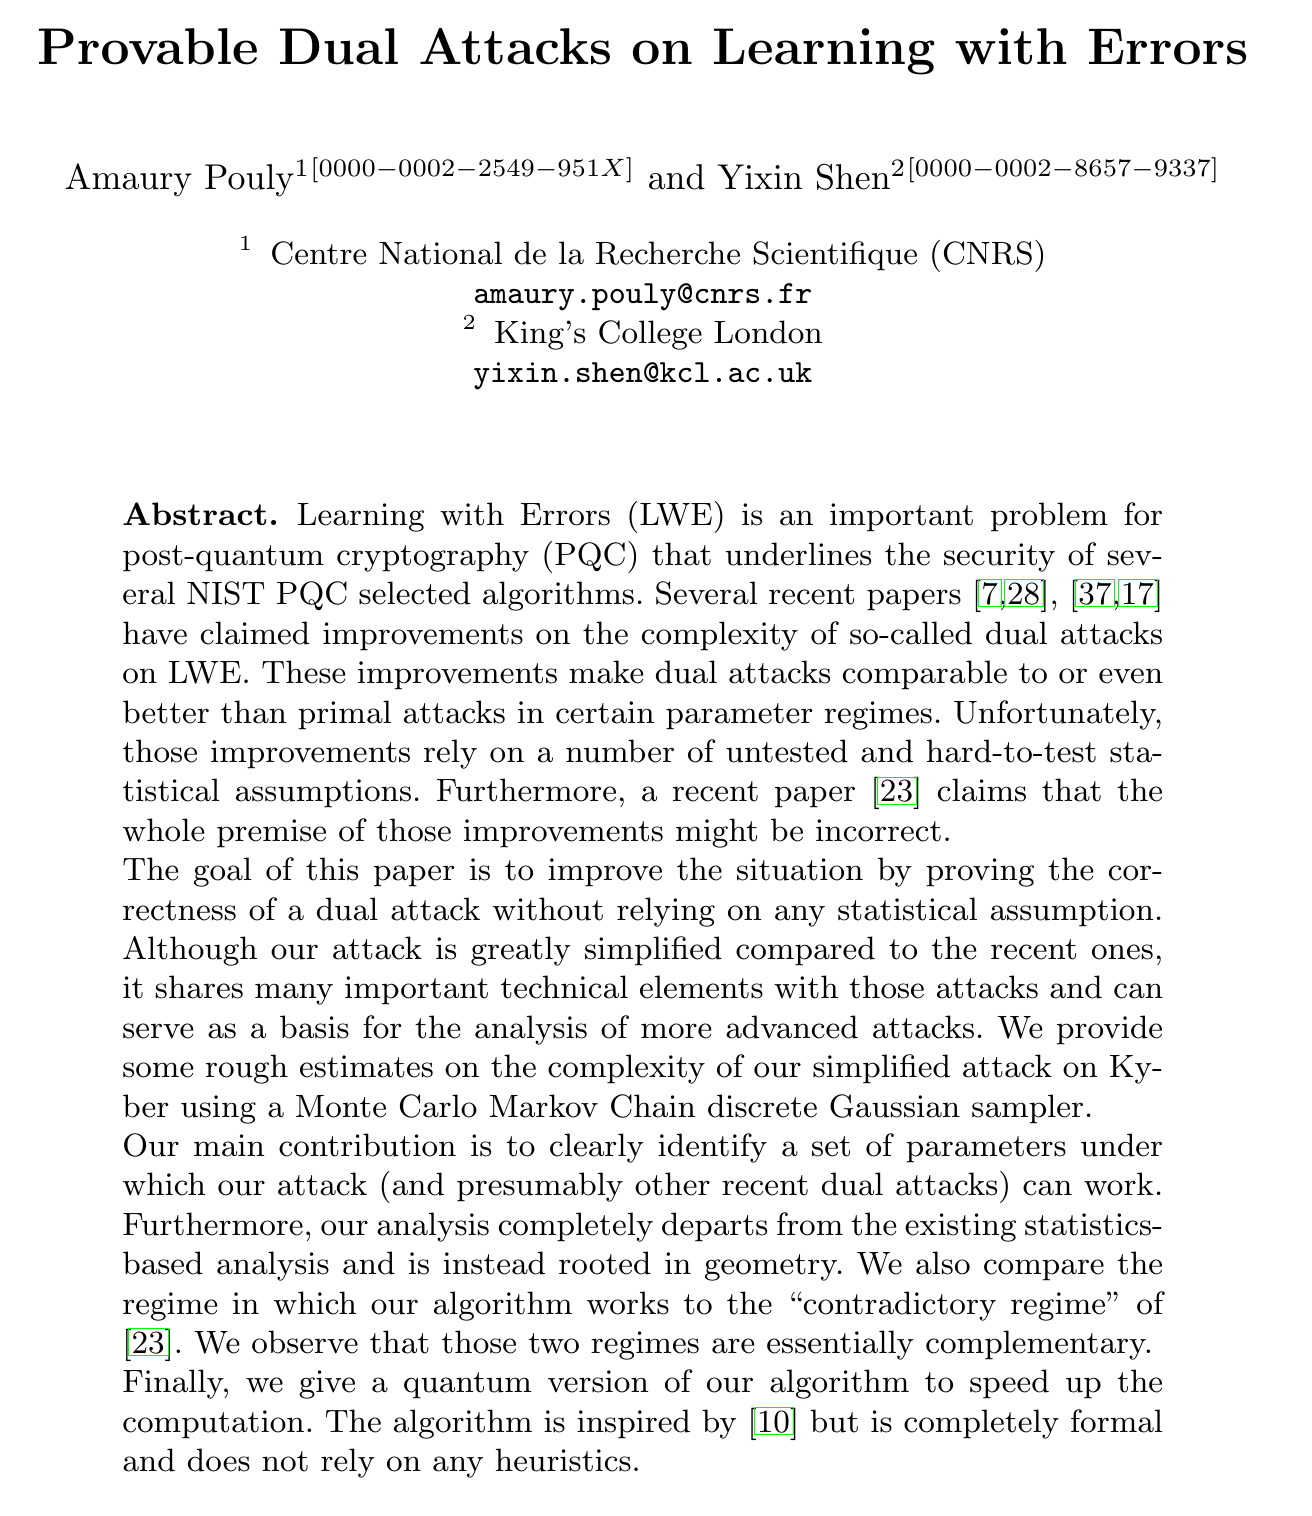
\includegraphics[keepaspectratio,height=.8\textheight]{./yixin.png}
\end{center}
\end{column}
\end{columns}
\end{frame}

\begin{frame}[label={sec:org33ddb80}]{Summary}
\begin{columns}[t]
\begin{column}{0.6\columnwidth}
\begin{itemize}
\item Heuristics used in dual-attack analysis are being cleaned up, community is gaining clarity on its expected performance
\item But this only treats statistical/geometric questions, but not computational costs
\begin{itemize}
\item See John's talk
\end{itemize}
\end{itemize}
\end{column}

\begin{column}{0.4\columnwidth}
\begin{itemize}
\item It seems \textbf{morally wrong} that the dual attack would beat the primal attack. If the universe is \textbf{just}, the somewhat direct approach \textbf{should} beat running lattice reduction on the transpose and computing inner products.
\end{itemize}
\end{column}
\end{columns}
\end{frame}

\begin{frame}[label={sec:orgd85b71f}]{ML Attacks}
\begin{columns}
\begin{column}[t]{0.5\columnwidth}
{\footnotesize

\begin{itemize}
\item \fullcite{NeurIPS:WCCL22}
\item \fullcite{CCS:LSWMGCL23}
\end{itemize}

\par}
\end{column}

\begin{column}[t]{0.5\columnwidth}
{\footnotesize

\begin{itemize}
\item \fullcite{EPRINT:LSWACL23}
\item \fullcite{EPRINT:SWLNSCL24}
\end{itemize}

\par}
\end{column}
\end{columns}
\end{frame}

\begin{frame}[allowframebreaks]{Claims}
\begin{quote}
\textbf{Ethics and Broader Impact.} The primary value of this work is in alerting the cryptographic and ML communities to the risk of ML-based attacks on PQC. Even if current attacks do not succeed, we believe that \alert{providing early warning of potential threats is critical}. However, we emphasize that SALSA represents a proof of concept that cannot be used against real-world implementations (i.e. the PQC schemes which NIST standardized on July 5, 2022). Additional scaling work would be necessary before these techniques would be relevant to attacking real-world cryptosystems.`` -- \cite{NeurIPS:WCCL22}
\end{quote}

\framebreak

\begin{quote}
\textbf{Ethical considerations.} Although Picante demonstrates significant progress towards attacking real-world LWE problems with sparse binary secrets, \alert{it cannot yet break} problems with real-world-size parameters. In particular, the LWE schemes standardized by NIST use smaller modulus q and non-sparse secret distributions. Hence, we do not believe our paper raises any ethical concerns. Nonetheless, we shared a copy of the current paper with the NIST Cryptography group, to inform them of our approach. --  \cite{CCS:LSWMGCL23}
\end{quote}

\framebreak

\begin{quote}
\textbf{Limitations and broader impact.} Despite significantly advancing the state-of-the-art in ML-based
LWE attacks, VERDE \alert{cannot yet break} standardized LWE-based PQC schemes, limiting its real-world
impact. Because of this, our paper raises no immediate security concerns. Nevertheless, we have
shared a copy of our paper with the NIST PQC group to make them aware of this attack. -- \cite{EPRINT:LSWACL23}
\end{quote}

\framebreak

\begin{quote}
\textbf{8. Impact Statement} The main ethical concern related to this work is the possibility of our attack compromising currently-deployed PQC system. However, \alert{at present, our proposed attack does not threaten current standardized systems}. If our attack scales to higher \(h\) and lower \(q\) settings, then its impact is significant, as it would necessitate changing PQC encryption standards. For reproducability of these results, our code will be open sourced after publication and is available to reviewers upon request. -- \cite{EPRINT:SWLNSCL24} 
\end{quote}
\end{frame}

\begin{frame}[label={sec:orgf4135eb}]{Attack Description}
\begin{columns}
\begin{column}{0.35\columnwidth}
\begin{center}
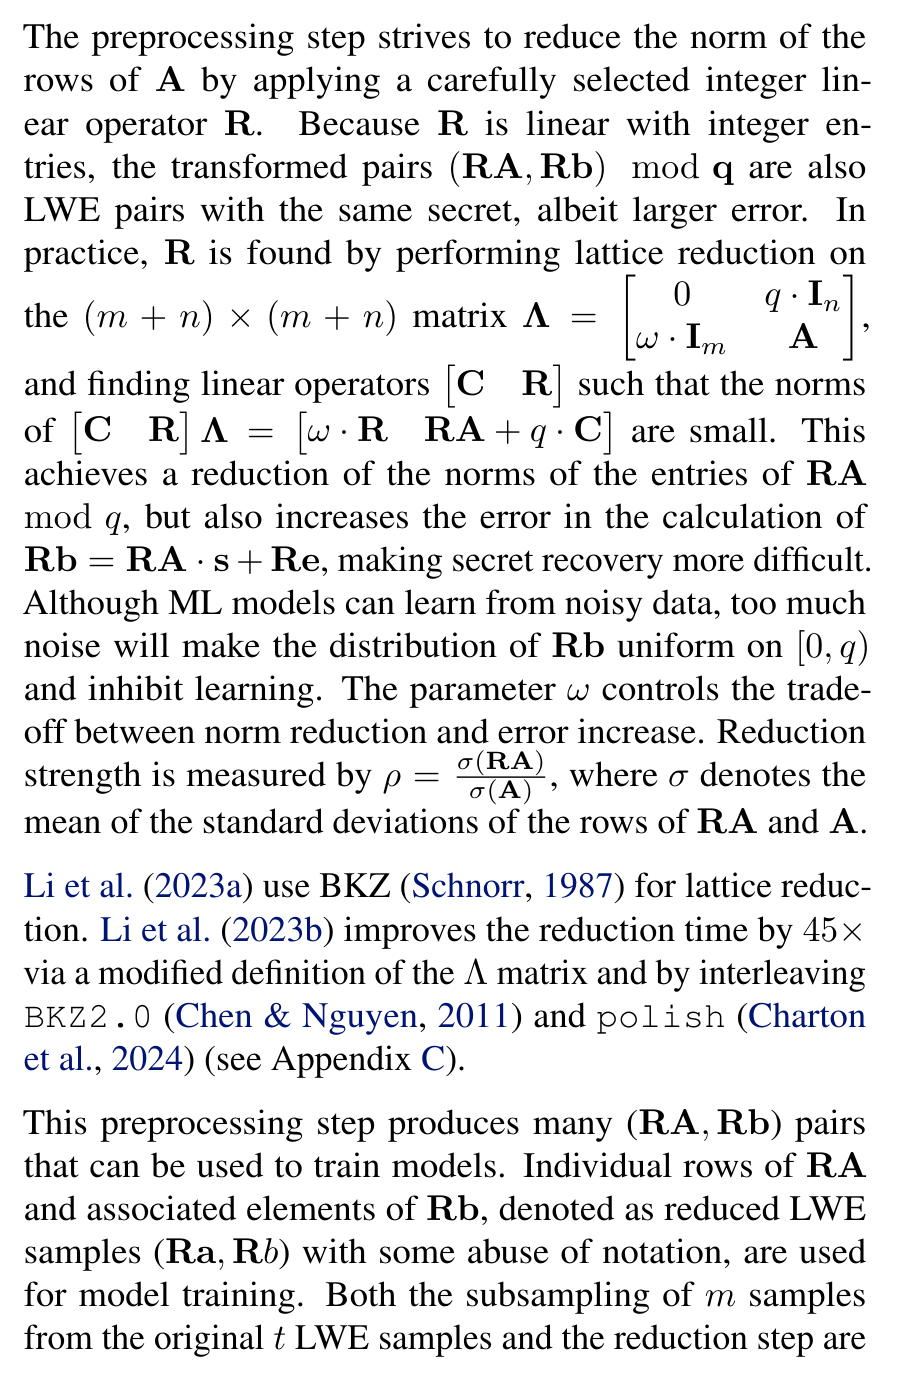
\includegraphics[width=.9\linewidth]{./salsa-fresca-algorithm.png}
\end{center}
\end{column}

\begin{column}{0.65\columnwidth}
Recent versions of the attack (VERDE/FRESCA) are essentially variants of the dual attack.

\begin{itemize}
\item \(\vec{u}^{T} \cdot \vec{c} \equiv \vec{u}^{T} \cdot \vec{A} \cdot \vec{s} + \vec{u}^{T} \cdot \vec{e} \equiv \vec{v}^{T} \cdot \vec{s} + \vec{u}^{T}\cdot \vec{e}\)  \(\Rightarrow\) \alert{short-ish}
\item \(\vec{u}^{T} \cdot \vec{c}\) \(\Rightarrow\) \alert{uniform}
\end{itemize}

\begin{block}{Distinguishers}
Modelling \(\vec{v}^{T} \cdot \vec{s} + \vec{u}^{T}\cdot \vec{e}\) as a discrete Gaussian mod \(q\) we can compute the statistical distance between these two distributions and thus the number of samples we need to distinguish with constant advantage.
\end{block}
\end{column}
\end{columns}
\end{frame}

\begin{frame}[label={sec:org77cb52b}]{Comparison with State of the Art: SALSA VERDE I}
\begin{center}
\includegraphics[keepaspectratio,page=3,frame,height=.7\textheight]{./crypto2023rump-paper13.pdf}
\end{center}

{\footnotesize \url{https://crypto.iacr.org/2023/rump/crypto2023rump-paper13.pdf} \par}
\end{frame}

\begin{frame}[label={sec:org63d9992}]{Comparison with State of the Art: SALSA VERDE II}
\begin{center}
\includegraphics[keepaspectratio,page=6,frame,height=.7\textheight]{./crypto2023rump-paper13.pdf}
\end{center}

{\footnotesize \url{https://crypto.iacr.org/2023/rump/crypto2023rump-paper13.pdf} \par}
\end{frame}

\begin{frame}[label={sec:org1395adf},fragile]{Comparison with Something: SALSA FESCA I}
 \begin{center}
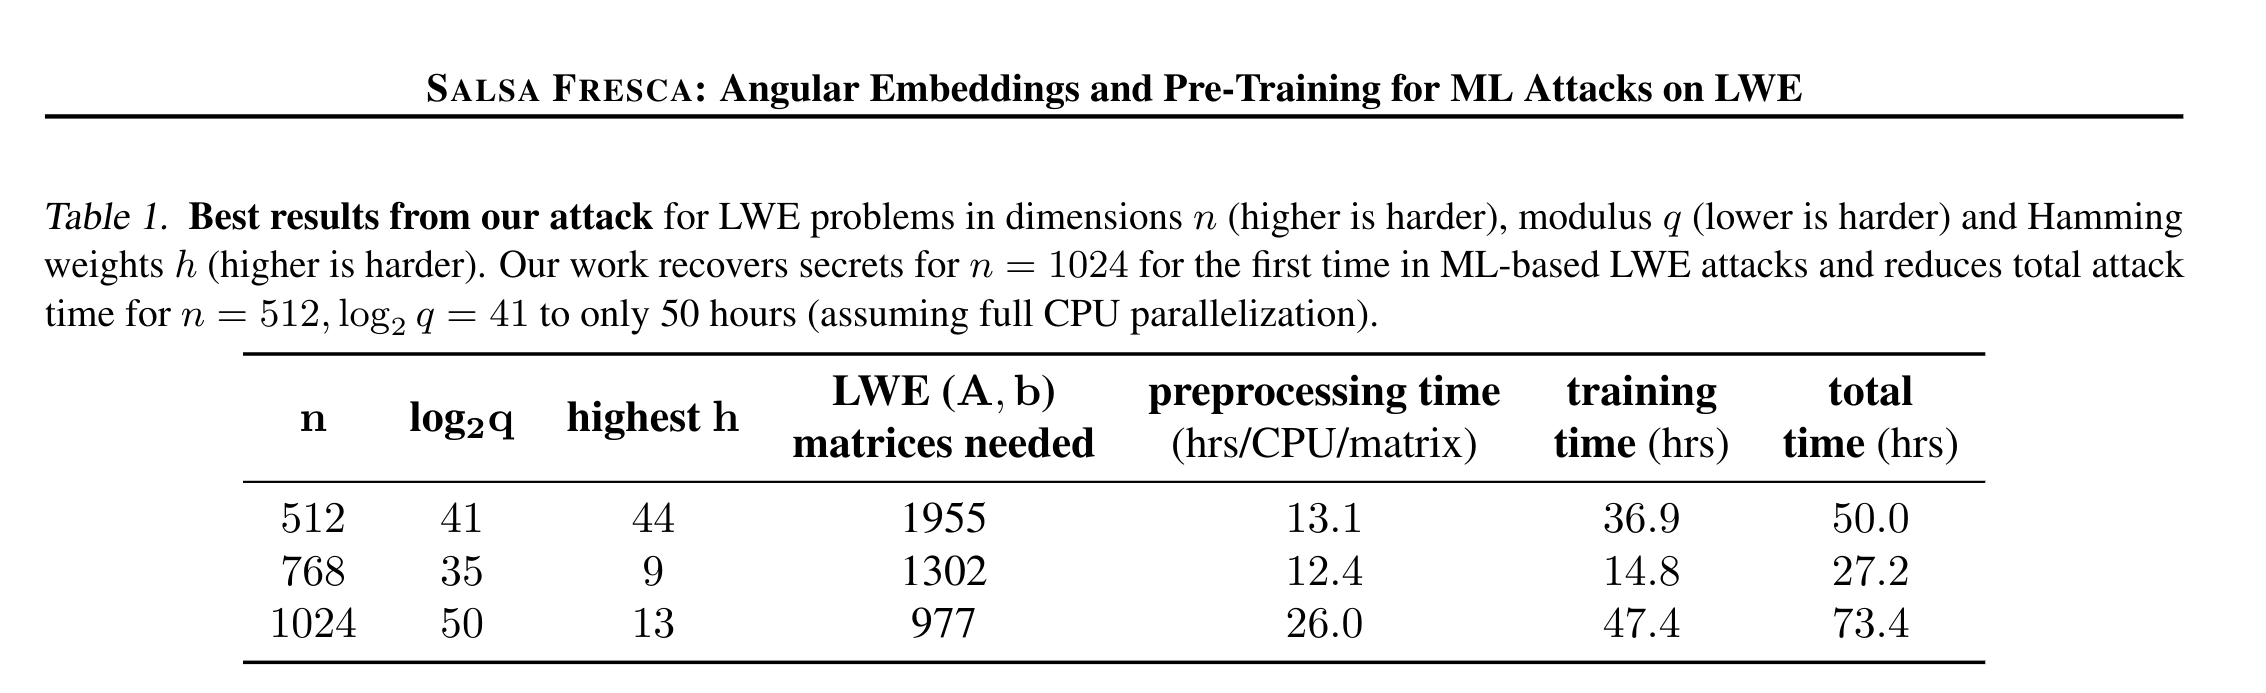
\includegraphics[width=.9\linewidth]{./salsa-fresca-results.png}
\end{center}

\begin{lstlisting}[language=Python,label= ,caption= ,captionpos=b,numbers=none]
from estimator import *
params = LWE.Parameters(n=1024, q=2^50, Xs=ND.SparseTernary(n=1024, p=7, m=7), Xe=ND.DiscreteGaussian(3))
LWE.primal_hybrid(params)
\end{lstlisting}

\begin{verbatim}
rop: ≈2^48.4, red: ≈2^48.1, svp: ≈2^46.2, β: 41, η: 2, ζ: 478, |S|: ≈2^42.6, d: 1213, prob: 0.189, ↻: 22, …
\end{verbatim}


\begin{center}
\(\approx 52\) hrs vs \(977 \cdot 26 + 47.4 \approx 25402\) hrs 
\end{center}
\end{frame}

\begin{frame}[label={sec:orged77d3a},fragile]{Comparison with \alert{Something}: SALSA FESCA II}
 The ``lattice estimator''\footnote{\url{https://github.com/malb/lattice-estimator}} picks \(\beta\) = 40 as a lower bound, it is not designed to handle such easy instances.

\begin{lstlisting}[language=Python,label= ,caption= ,captionpos=b,numbers=none]
with local_minimum(40, max(2 * params.n, 41), precision=5) as it:
    for beta in it:
        cost = self.cost_gsa(
            beta=beta, params=params, m=m, red_cost_model=red_cost_model, **kwds
        )
        it.update(cost)
    for beta in it.neighborhood:
        cost = self.cost_gsa(
            beta=beta, params=params, m=m, red_cost_model=red_cost_model, **kwds
        )
        it.update(cost)
    cost = it.y
\end{lstlisting}

{\footnotesize \url{https://github.com/malb/lattice-estimator/blob/main/estimator/lwe\_primal.py\#L209-L220} \par}
\end{frame}

\begin{frame}[label={sec:org36b881b}]{High-Level}
There is no particular reason to believe that ML can threaten LWE.

\begin{columns}
\begin{column}{0.6\columnwidth}
\begin{center}
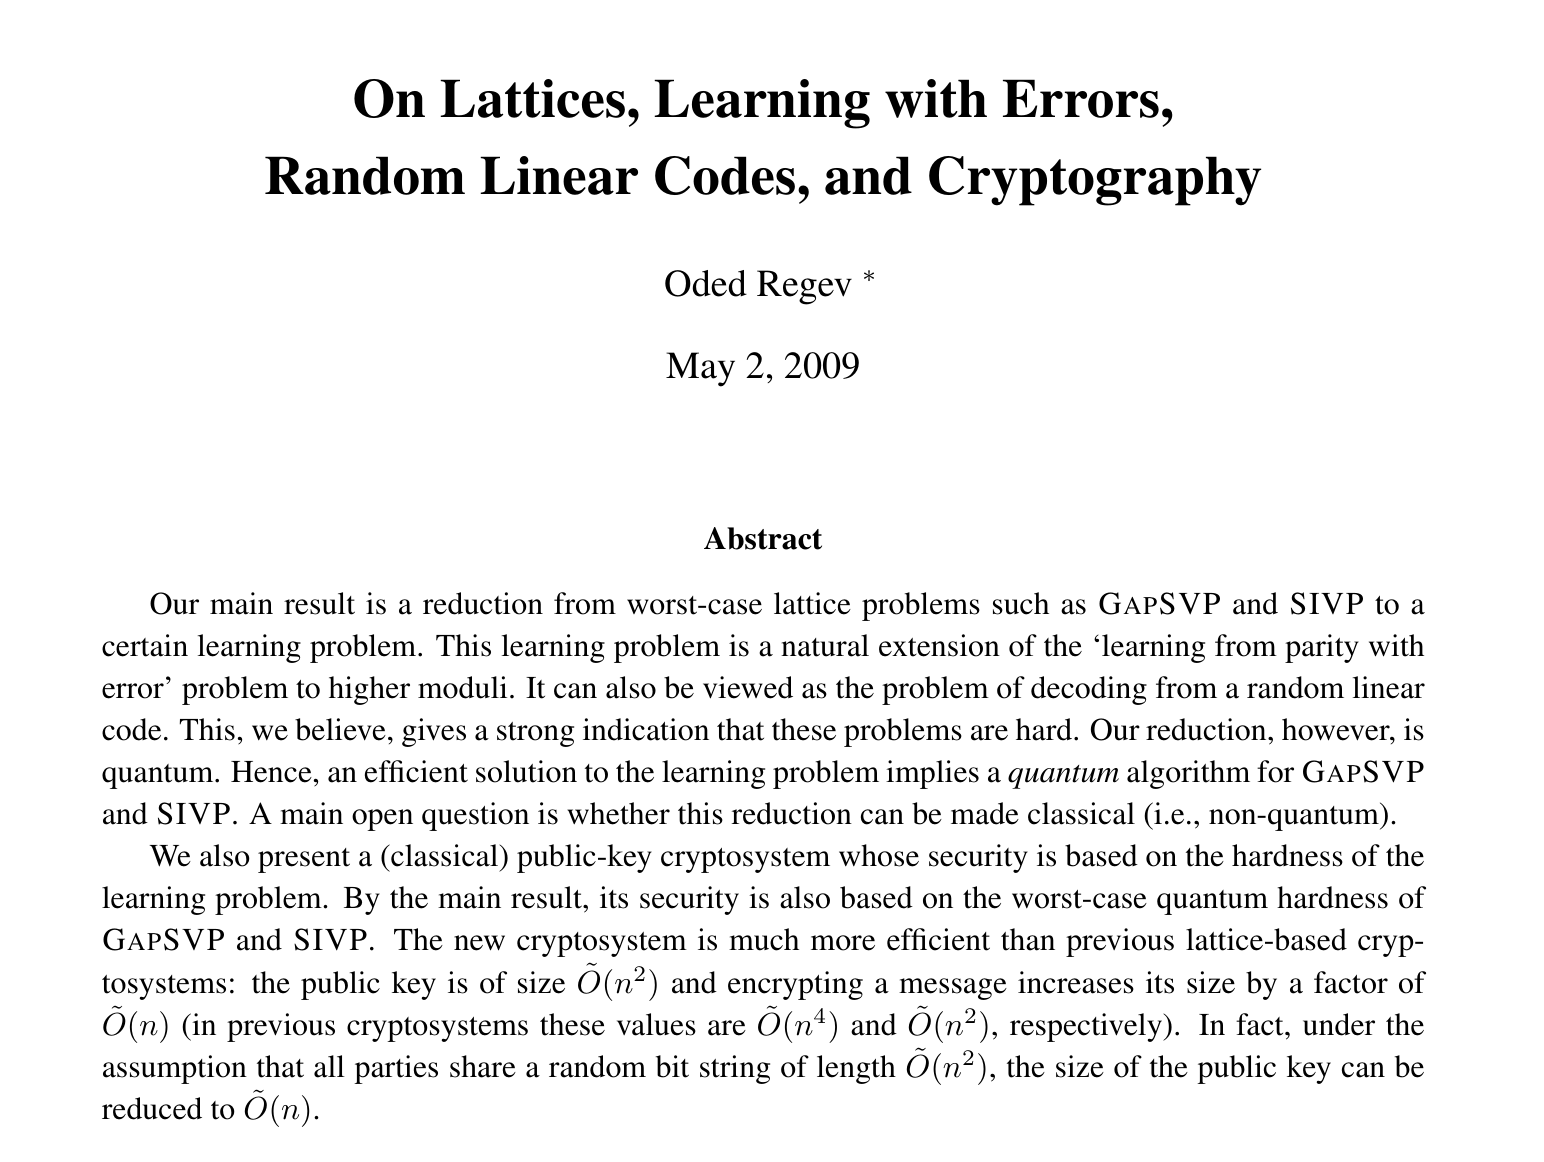
\includegraphics[width=.9\linewidth]{./regev-hard-learning-problems.png}
\end{center}
\end{column}


\begin{column}{0.4\columnwidth}
\begin{itemize}
\item \textbf{LWE} is (designed to be) a hard learning problem.
\item \textbf{ML} classifiers exploit statistical patterns in the data.\footnote{This is a reason why they work somewhat well on e.g. side-channel traces.}
\end{itemize}

\begin{alertblock}{Open Problem}
Not easy to establish the state of the art for LWE instances within range of experiments. More advanced algorithms lack efficient, versatile and public implementations.
\end{alertblock}
\end{column}
\end{columns}
\end{frame}

\begin{frame}[label={sec:org321b4fa},standout]{Fin \& Obligatory ``We're hiring'' Slide}
\begin{center}
\Huge \alert{Thank You}
\end{center}

\begin{description}
\item[{KCL}] Academic staff, postdocs and PhD students (all areas of cryptography)
\item[{SandboxAQ}] Postdoc/PhD/FTEs/Consultants: PQC PhD residencies, PQC Postdocs, Cryptography SWE
\end{description}
\end{frame}

\begin{frame}[allowframebreaks]{References}
\renewcommand*{\bibfont}{\scriptsize}
\printbibliography[heading=none]
\end{frame}
\end{document}
